% main.tex — arXiv preprint, English edition.
% Compile: pdflatex main && bibtex main && pdflatex main && pdflatex main
% (or: latexmk -pdf main)

\documentclass[11pt,a4paper]{article}

% ---- Packages ----------------------------------------------------------
\usepackage[utf8]{inputenc}
\usepackage[T1]{fontenc}
\usepackage{lmodern}
\usepackage[a4paper,margin=1in]{geometry}
\usepackage{microtype}
\usepackage{authblk}
\usepackage{amsmath,amssymb}
\usepackage{booktabs}
\usepackage{tabularx}
\usepackage{array}
\usepackage{multirow}
\usepackage{enumitem}
\usepackage{verbatim}
\usepackage{fancyvrb}
\usepackage{url}
\usepackage{xcolor}
\usepackage{graphicx}
\usepackage{tikz}
\usetikzlibrary{arrows.meta,positioning,shapes.geometric,calc,fit}
\usepackage{caption}
\usepackage{listings}
\usepackage{hyperref}
\hypersetup{
  colorlinks=true,
  linkcolor=blue!50!black,
  citecolor=blue!50!black,
  urlcolor=blue!50!black,
}
\usepackage[capitalize,nameinlink]{cleveref}

% Code listings
\lstset{
  basicstyle=\ttfamily\footnotesize,
  breaklines=true,
  columns=fullflexible,
  showstringspaces=false,
  frame=single,
  framesep=4pt,
  rulecolor=\color{gray!40},
  backgroundcolor=\color{gray!4},
}

% Tighten lists slightly
\setlist{topsep=2pt,partopsep=0pt,itemsep=2pt,parsep=0pt}

% ---- Title ------------------------------------------------------------
\title{Measuring Model Substitution in OpenAI-Compatible API Resellers:\\
  A 14-Day Study of 171 Endpoints}

\author[1]{Bazaarlink Research}
\affil[1]{\texttt{bazaarlink.ai} --- corresponding repository: \\
  \url{https://github.com/Bazaarlinkorg/LLMprobe-engine}}

\date{2026-04-26 (arXiv-v1)}

% ---- Document --------------------------------------------------------
\begin{document}
\maketitle

% =====================================================================
\begin{abstract}
The market for resold access to large-language-model (LLM) APIs has expanded
rapidly since 2024, driven by upstream providers' regional service-availability
policies. Because upstream providers cannot authenticate which back-end model a
third-party reseller actually routes to, and because protocol-layer responses
are nearly indistinguishable across models, downstream buyers cannot directly
detect silent model substitution. We design a four-layer black-box detection
system based on independent behavioral fingerprints: a surface family
classifier, a behavior column with self-claim zeroed, a sub-model deterministic
match (cutoff / capability / refusal-prefix), and a behavioral-vector extension
covering refusal-boundary ladder, formatting idiosyncrasy, and calibrated
uncertainty. We apply it to 171 distinct reseller endpoints over a 14-day
window (2026-04-12 to 2026-04-25; 625 probe runs). On cost-constrained
synthetic stress tests the system achieves 94.4\% intra-family true-positive
rate ($n{=}18$; Wilson 95\% CI $[74.2\%, 99.0\%]$) at 0\% false-positive rate
($n{=}6$). In the field, \textbf{9.9\% of probed endpoints (17/171) show at
least one detected substitution event; under a stricter criterion ($n{\geq}5$
probes, ${\geq}20\%$ violation rate) 1.3\% (2/149) exhibit persistent
substitution}. Observed substitutions sort into five categories: cross-family
impersonation, silent downgrade, silent upgrade, version-tag forgery, and
provider-injected behavioral constraint. We complement Liu et al.\
(arXiv:2604.08407)~\cite{liu2026agent} ---  who measure malicious-intermediary
security attacks on the LLM supply chain --- by quantifying the orthogonal axis
of model-substitution quality fraud, and close with three disclosure-duty
proposals.

\medskip
\noindent\textbf{Keywords:} LLM API resale; model substitution; behavioral
fingerprinting; consumer protection; black-box auditing.
\end{abstract}

% =====================================================================
\section*{Disclosure and Ethics Statement}

\paragraph{Authors' relationship to the deployed system.}
The authors operate the public Web service \texttt{bazaarlink.ai/probe}
referred to in \cref{sec:impl}. The detection methodology described in this
paper is released under AGPL-3.0 as the open-source package
\texttt{@bazaarlink/probe-engine} (see \cref{app:opensource}); the SaaS
deployment is \emph{not} required to reproduce the methodology or any result
reported in \cref{sec:results}.

\paragraph{Measurement ethics.}
All probe traffic was issued via legitimately purchased API keys, of the same
class any retail customer of the studied endpoints could issue. The study
performed no denial-of-service, no billing-bypass, no unauthorized access, and
no action exceeding the access scope advertised by the endpoints. Every named
endpoint is a publicly marketed reseller of LLM API credit and was, throughout
the measurement window, receiving research-purpose stress-test traffic in
support of methodology validation; the substitution behaviors documented in
this paper are independent of that stress-test traffic.

\paragraph{Endpoint identification.}
Endpoints are referred to in the body of the paper by codenames (R1--R15) with
partial-letter masking of their domains. The full codename--domain mapping is
preserved in the authors' internal records and is \textbf{not} included as a
public appendix in this arXiv version; bona-fide researchers may request access
via the corresponding repository at\\
\url{https://github.com/Bazaarlinkorg/LLMprobe-engine}.

\paragraph{IRB.}
This study did not require Institutional Review Board approval because it does
not involve human subjects; all measured systems are publicly marketed API
services. The authors followed the spirit of the ACM Code of Ethics; a
self-assessment is documented in \cref{sec:irb}.

\paragraph{Position statement.}
The study aims at consumer protection and market transparency. It does not
make legal claims about any operating entity behind the studied endpoints.

% =====================================================================
\section{Introduction}\label{sec:intro}

\subsection{A market born of access restrictions}
Anthropic and OpenAI publicly disclose, in their service terms and acceptable-use
policies~\cite{anthropic2026aup,openai2026usage}, that their flagship products
are unavailable for direct purchase in certain countries and regions. Demand
for these tools has not abated in those regions; the productivity arms race
between developers in restricted regions and their global peers has, if
anything, intensified the demand. The supply--demand gap so created has, over
the past twelve months, given rise to a high-growth resale industry: third-party
operators stand up OpenAI-compatible HTTP endpoints in accessible jurisdictions,
back the endpoints with first-party API keys, and resell access at a markup to
downstream users in restricted regions. Such resale endpoints typically
advertise support for flagship models (Claude Opus 4.7, GPT-5.4, Gemini 3.1
Pro), and present an OpenAI-compatible interface so that downstream code
originally targeted at first-party SDKs may switch over without modification.

This is not the familiar pattern of a sanctioned API reseller. Sanctioned
resellers (e.g., on cloud-marketplaces) typically have formal contracts with
the upstream provider, contractual SLAs, and an interface that surfaces the
upstream provenance. The resellers studied in this paper instead operate as
\emph{unauthorized gray-market intermediaries}: upstream providers have not
authorized resale, the resellers' upstream API keys cannot be reconciled to
downstream buyers in the upstream's books, and downstream users routinely
\emph{assume} service homogeneity from interface compatibility.

\subsection{The collapse of trust assumptions}
Downstream buyers' trust in such intermediaries traditionally rests on four
assumptions: (1)~\textbf{interface}: the endpoint implements the
OpenAI-compatible protocol, therefore its behavior approximates first-party;
(2)~\textbf{self-claim}: a request that passes \texttt{model: claude-opus-4-7}
and receives a response self-identifying as Claude indicates the back end truly
is that model; (3)~\textbf{branding}: a website displaying upstream logos and
customer service claiming ``official partnership'' sources from the official
upstream; (4)~\textbf{pricing}: resellers will not collect high-tier model fees
while routing to a low-tier model. We will demonstrate that all four
assumptions fail in the present resale market.

\subsection{Research questions}
\textbf{RQ1 (Prevalence)} What fraction of currently active LLM API reseller
endpoints exhibit externally observable model substitution?
\textbf{RQ2 (Typology)} Can the observed substitution behaviors be organized
into reproducible categories?
\textbf{RQ3 (Detection feasibility)} Under purely black-box observation, can a
detection method achieve simultaneously high true-positive rate and low
false-positive rate?
\textbf{RQ4 (Consumer impact)} What concrete harms does substitution impose on
downstream buyers, and what are the implications for regulators and upstream
providers?

\subsection{Contributions and relation to prior work}
The contributions are: (1) a first systematic measurement of the resale market
for model-substitution behavior; (2) a reproducible black-box detection
methodology achieving 94.4\% intra-family TP at 0\% FP under cost-constrained
synthetic tests; (3) a five-category taxonomy of substitution behaviors; (4) a
consumer-protection policy analysis with three immediately implementable
disclosure-duty proposals.

\paragraph{Relation to prior work.}
The closest contemporary measurement is Liu et al.~\cite{liu2026agent}, who
measure 428 LLM API routers for \emph{active security attacks}: payload
injection, secret/credential exfiltration, evasion tactics, and crypto-asset
access. Our work measures the orthogonal axis: routers that perform
\emph{passive quality substitution} --- silently routing a paid-for premium
model to a cheaper or different one --- without active intrusion on the user's
system. Together, the two studies span the principal threat surfaces of the
LLM API supply chain: Liu et al.\ on what the router does \emph{to the user},
and the present paper on what the router does \emph{with the model}.

For the technical building blocks of layer~\textcircled{4} (\cref{sec:layer4})
we draw on three threads. The refusal-boundary ladder is informed by
mechanistic work on refusal direction in safety-tuned
LLMs~\cite{arditi2024refusal}. The formatting fingerprint follows the
observation that stylistic preferences are pre-training-baked and resist
runtime instruction~\cite{mcgovern2024stylistic}. The calibrated-uncertainty
channel applies the round-rate intuition from Kadavath et al.'s study of LLM
self-knowledge~\cite{kadavath2022know}. The deterministic sub-model matcher of
layer~\textcircled{3} extends behavioral fingerprinting along the lines of
LLMmap~\cite{pasquini2024llmmap} but adapts it to within-family discrimination
rather than across-family identification. The economic framing in
\cref{sec:policy} builds on Akerlof's seminal analysis of asymmetric
information in markets where quality is unobservable to
buyers~\cite{akerlof1970lemons}. Methodological design draws on Paxson's
framework for sound Internet measurement~\cite{paxson2004sound}.

\subsection{Structure}
\Cref{sec:threat} lays out the threat model. \Cref{sec:method} describes the
four-layer detection method. \Cref{sec:impl} outlines the engineering
implementation. \Cref{sec:results} reports synthetic and field measurement
results. \Cref{sec:taxonomy} organizes substitution behaviors into a taxonomy
with anchor cases including three deep case studies (R1, R2, R6).
\Cref{sec:policy} analyzes consumer harm and policy implications.
\Cref{sec:discussion} discusses limitations. \Cref{sec:conclusion} concludes.

% =====================================================================
\section{Threat Model}\label{sec:threat}

\subsection{Adversary types}
We classify substitution-capable adversaries (resellers) by commercial motivation:

\begin{itemize}
\item \textbf{Arbitrage adversary.} Advertises model $M_{\text{high}}$; routes
  to a cheaper same-family model $M_{\text{low}}$ (e.g., advertises Opus 4.7,
  routes to Sonnet 4.6). Motivation: per-token cost differential $\times$ volume.
\item \textbf{Silent-downgrade adversary.} Advertises $M_{\text{high}}$ and
  initially routes to $M_{\text{high}}$, but switches to $M_{\text{low}}$ under
  operational pressure (cost squeeze, upstream-quota exhaustion).
\item \textbf{Cross-family adversary.} Advertises a model in family $F_a$
  (Anthropic Claude); routes to a model in family $F_b$ (OpenAI GPT, Google
  Gemini, Z-AI GLM). Motivation: cross-family arbitrage, or fail-over when
  $F_a$ accounts are blocked.
\end{itemize}

A non-pecuniary fourth pattern is observed:

\begin{itemize}
\item \textbf{Behavior-injection adversary.} Injects a system prompt at the
  upstream layer (e.g., Amazon Q Developer / Kiro coding-agent wrapper) that
  constrains an otherwise general-purpose model to a narrow domain. Downstream
  users do receive the advertised model, but its behavioral freedom is
  silently restricted.
\end{itemize}

\subsection{Adversary capabilities}
The adversary has full control over: request routing (upstream key + model
parameter), request rewriting (system prompt injection), response rewriting,
header injection, and streaming forgery. The adversary does \emph{not} possess
the ability to rewrite the upstream model's internal reasoning (logprobs,
token-count physics) or to forge the full behavioral fingerprint of an upstream
model in absence of that model's participation. The adversary may rewrite
\emph{what the response says}, but cannot at low cost fabricate a coherent set
of responses spanning multiple independent fingerprint channels.

\subsection{Attack-surface classification}
Mapping the substitution to its injection point in the request lifecycle:

\begin{table}[h]
\centering
\small
\begin{tabular}{@{}lll@{}}
\toprule
Surface & Injection point & Forgery ceiling \\
\midrule
Routing layer & upstream key / \texttt{model} & full back-end replacement \\
Prompt layer & upstream system prompt & forge self-claim; not refusal floor \\
Response layer & post-process upstream response & rewrite text; not metadata \\
\bottomrule
\end{tabular}
\end{table}

% =====================================================================
\section{Methodology: Four-Layer Independent Fingerprint Detection}\label{sec:method}

\subsection{Design principles}
\textbf{P1 Multi-layer independence.} Each detection layer uses an independent
signal channel; an adversary must simultaneously forge consistent behavior
across channels to escape detection.
\textbf{P2 Black-box accessibility.} All channels are obtained via downstream
HTTP API alone; no privileged access is required.
\textbf{P3 Quantified confidence.} The system outputs not only a Boolean
verdict but a quantified confidence band and per-layer evidence trail.

\subsection{Architecture overview}\label{sec:arch}
% fig-architecture.tex — Figure 1: Four-layer detection architecture
% Self-contained TikZ figure. Compile with pdflatex/xelatex/lualatex.
% Used by main.tex via % fig-architecture.tex — Figure 1: Four-layer detection architecture
% Self-contained TikZ figure. Compile with pdflatex/xelatex/lualatex.
% Used by main.tex via % fig-architecture.tex — Figure 1: Four-layer detection architecture
% Self-contained TikZ figure. Compile with pdflatex/xelatex/lualatex.
% Used by main.tex via \input{fig-architecture}.

\begin{figure}[t]
\centering
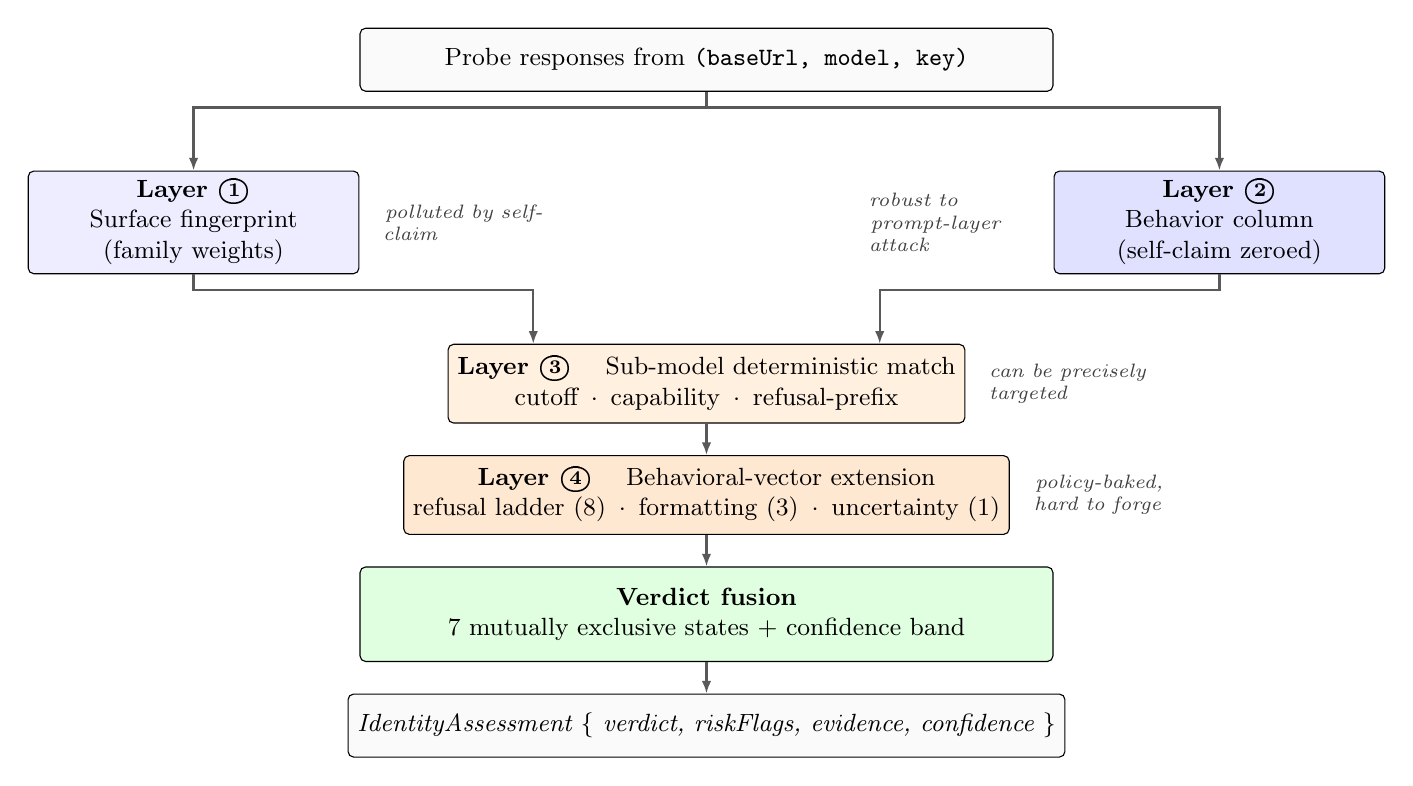
\begin{tikzpicture}[
  node distance=4mm and 6mm,
  every node/.style={font=\small},
  layer/.style={
    draw, rounded corners=2pt,
    minimum width=42mm, minimum height=10mm,
    align=center, fill=gray!8,
  },
  surface/.style={layer, fill=blue!7},
  behavior/.style={layer, fill=blue!12},
  v3/.style={layer, fill=orange!12},
  v3e/.style={layer, fill=orange!18},
  fusion/.style={layer, fill=green!12, minimum width=88mm, minimum height=12mm},
  input/.style={
    draw, rounded corners=2pt,
    minimum width=88mm, minimum height=8mm,
    align=center, fill=gray!4,
  },
  output/.style={
    draw, rounded corners=2pt,
    minimum width=88mm, minimum height=8mm,
    align=center, fill=gray!4,
    font=\small\itshape,
  },
  arrow/.style={-{Latex[length=1.6mm]}, thick, gray!70!black},
  label/.style={font=\scriptsize\itshape, gray!50!black},
]

% Top: input
\node[input] (input) {Probe responses from \texttt{(baseUrl, model, key)}};

% Layer 1 + Layer 2 side by side
\node[surface, below left=10mm and 0mm of input] (l1) {%
  \textbf{Layer \textcircled{\scriptsize 1}}\\Surface fingerprint\\(family weights)};
\node[behavior, below right=10mm and 0mm of input] (l2) {%
  \textbf{Layer \textcircled{\scriptsize 2}}\\Behavior column\\(self-claim zeroed)};

% Layer 3 below
\node[v3, below=10mm of input, yshift=-22mm] (l3) {%
  \textbf{Layer \textcircled{\scriptsize 3}} \quad Sub-model deterministic match\\
  cutoff $\,\cdot\,$ capability $\,\cdot\,$ refusal-prefix};
\path (l3.west) -- node[layer, minimum width=88mm, draw=none, fill=none] {} (l3.east);

% Layer 4 below
\node[v3e, below=4mm of l3] (l4) {%
  \textbf{Layer \textcircled{\scriptsize 4}} \quad Behavioral-vector extension\\
  refusal ladder (8) $\,\cdot\,$ formatting (3) $\,\cdot\,$ uncertainty (1)};

% Verdict fusion
\node[fusion, below=4mm of l4] (fuse) {%
  \textbf{Verdict fusion}\\
  7 mutually exclusive states + confidence band};

% Output
\node[output, below=4mm of fuse] (out) {%
  IdentityAssessment \{ verdict, riskFlags, evidence, confidence \}};

% Arrows
\draw[arrow] (input.south) -- ++(0,-2mm) -| (l1.north);
\draw[arrow] (input.south) -- ++(0,-2mm) -| (l2.north);
\draw[arrow] (l1.south) -- ++(0,-2mm) -| ([xshift=-22mm]l3.north);
\draw[arrow] (l2.south) -- ++(0,-2mm) -| ([xshift=22mm]l3.north);
\draw[arrow] (l3.south) -- (l4.north);
\draw[arrow] (l4.south) -- (fuse.north);
\draw[arrow] (fuse.south) -- (out.north);

% Side annotations
\node[label, right=2mm of l1, anchor=west, text width=20mm] {polluted by self-claim};
\node[label, left=2mm of l2, anchor=east, text width=20mm] {robust to prompt-layer attack};
\node[label, right=2mm of l3, anchor=west, text width=20mm] {can be precisely targeted};
\node[label, right=2mm of l4, anchor=west, text width=20mm] {policy-baked, hard to forge};

\end{tikzpicture}
\caption{The four-layer independent-fingerprint detection architecture (\S\ref{sec:method}).
Each layer uses an independent signal channel; an adversary must simultaneously forge
consistent behavior across multiple channels to escape detection. The verdict fusion
emits one of seven mutually exclusive states with a confidence band.}
\label{fig:architecture}
\end{figure}
.

\begin{figure}[t]
\centering
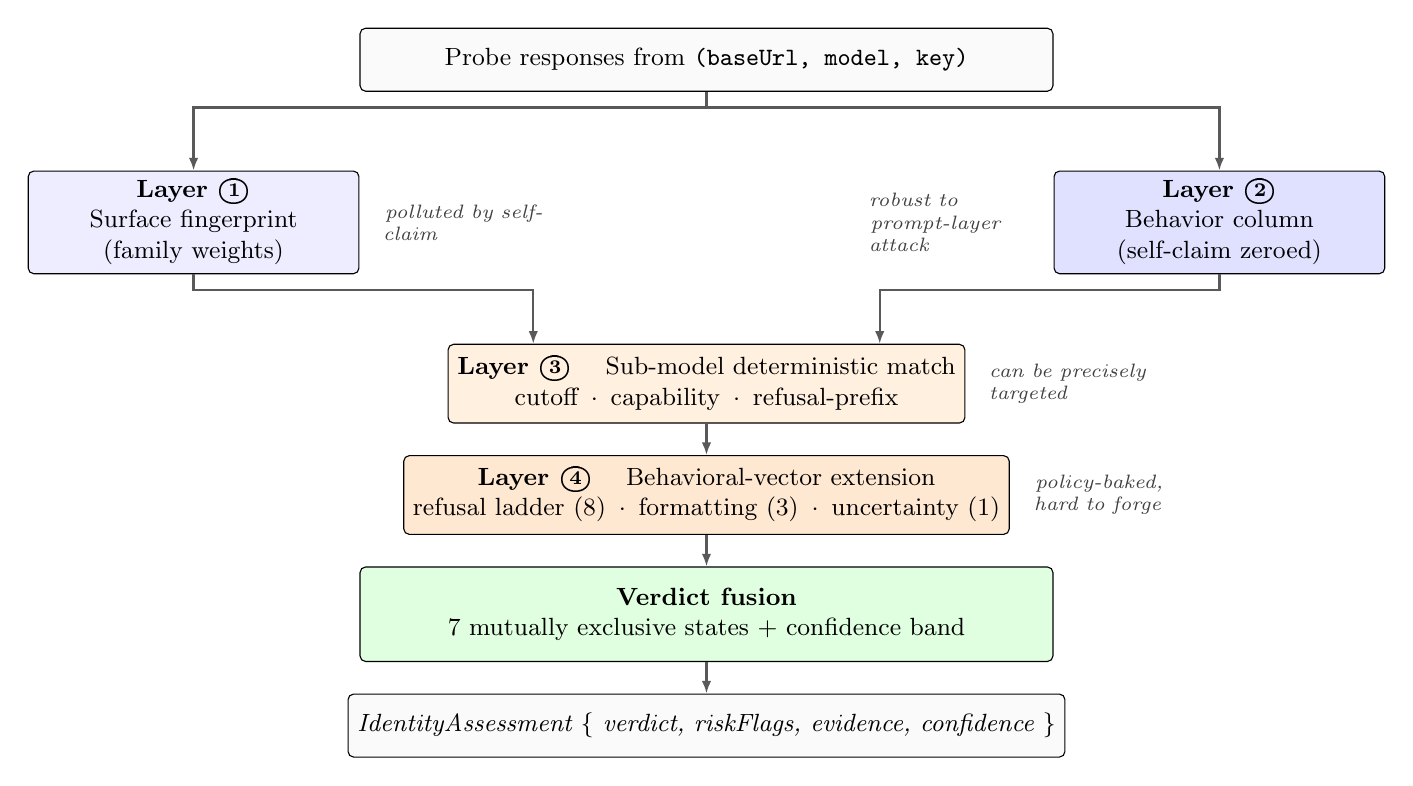
\begin{tikzpicture}[
  node distance=4mm and 6mm,
  every node/.style={font=\small},
  layer/.style={
    draw, rounded corners=2pt,
    minimum width=42mm, minimum height=10mm,
    align=center, fill=gray!8,
  },
  surface/.style={layer, fill=blue!7},
  behavior/.style={layer, fill=blue!12},
  v3/.style={layer, fill=orange!12},
  v3e/.style={layer, fill=orange!18},
  fusion/.style={layer, fill=green!12, minimum width=88mm, minimum height=12mm},
  input/.style={
    draw, rounded corners=2pt,
    minimum width=88mm, minimum height=8mm,
    align=center, fill=gray!4,
  },
  output/.style={
    draw, rounded corners=2pt,
    minimum width=88mm, minimum height=8mm,
    align=center, fill=gray!4,
    font=\small\itshape,
  },
  arrow/.style={-{Latex[length=1.6mm]}, thick, gray!70!black},
  label/.style={font=\scriptsize\itshape, gray!50!black},
]

% Top: input
\node[input] (input) {Probe responses from \texttt{(baseUrl, model, key)}};

% Layer 1 + Layer 2 side by side
\node[surface, below left=10mm and 0mm of input] (l1) {%
  \textbf{Layer \textcircled{\scriptsize 1}}\\Surface fingerprint\\(family weights)};
\node[behavior, below right=10mm and 0mm of input] (l2) {%
  \textbf{Layer \textcircled{\scriptsize 2}}\\Behavior column\\(self-claim zeroed)};

% Layer 3 below
\node[v3, below=10mm of input, yshift=-22mm] (l3) {%
  \textbf{Layer \textcircled{\scriptsize 3}} \quad Sub-model deterministic match\\
  cutoff $\,\cdot\,$ capability $\,\cdot\,$ refusal-prefix};
\path (l3.west) -- node[layer, minimum width=88mm, draw=none, fill=none] {} (l3.east);

% Layer 4 below
\node[v3e, below=4mm of l3] (l4) {%
  \textbf{Layer \textcircled{\scriptsize 4}} \quad Behavioral-vector extension\\
  refusal ladder (8) $\,\cdot\,$ formatting (3) $\,\cdot\,$ uncertainty (1)};

% Verdict fusion
\node[fusion, below=4mm of l4] (fuse) {%
  \textbf{Verdict fusion}\\
  7 mutually exclusive states + confidence band};

% Output
\node[output, below=4mm of fuse] (out) {%
  IdentityAssessment \{ verdict, riskFlags, evidence, confidence \}};

% Arrows
\draw[arrow] (input.south) -- ++(0,-2mm) -| (l1.north);
\draw[arrow] (input.south) -- ++(0,-2mm) -| (l2.north);
\draw[arrow] (l1.south) -- ++(0,-2mm) -| ([xshift=-22mm]l3.north);
\draw[arrow] (l2.south) -- ++(0,-2mm) -| ([xshift=22mm]l3.north);
\draw[arrow] (l3.south) -- (l4.north);
\draw[arrow] (l4.south) -- (fuse.north);
\draw[arrow] (fuse.south) -- (out.north);

% Side annotations
\node[label, right=2mm of l1, anchor=west, text width=20mm] {polluted by self-claim};
\node[label, left=2mm of l2, anchor=east, text width=20mm] {robust to prompt-layer attack};
\node[label, right=2mm of l3, anchor=west, text width=20mm] {can be precisely targeted};
\node[label, right=2mm of l4, anchor=west, text width=20mm] {policy-baked, hard to forge};

\end{tikzpicture}
\caption{The four-layer independent-fingerprint detection architecture (\S\ref{sec:method}).
Each layer uses an independent signal channel; an adversary must simultaneously forge
consistent behavior across multiple channels to escape detection. The verdict fusion
emits one of seven mutually exclusive states with a confidence band.}
\label{fig:architecture}
\end{figure}
.

\begin{figure}[t]
\centering
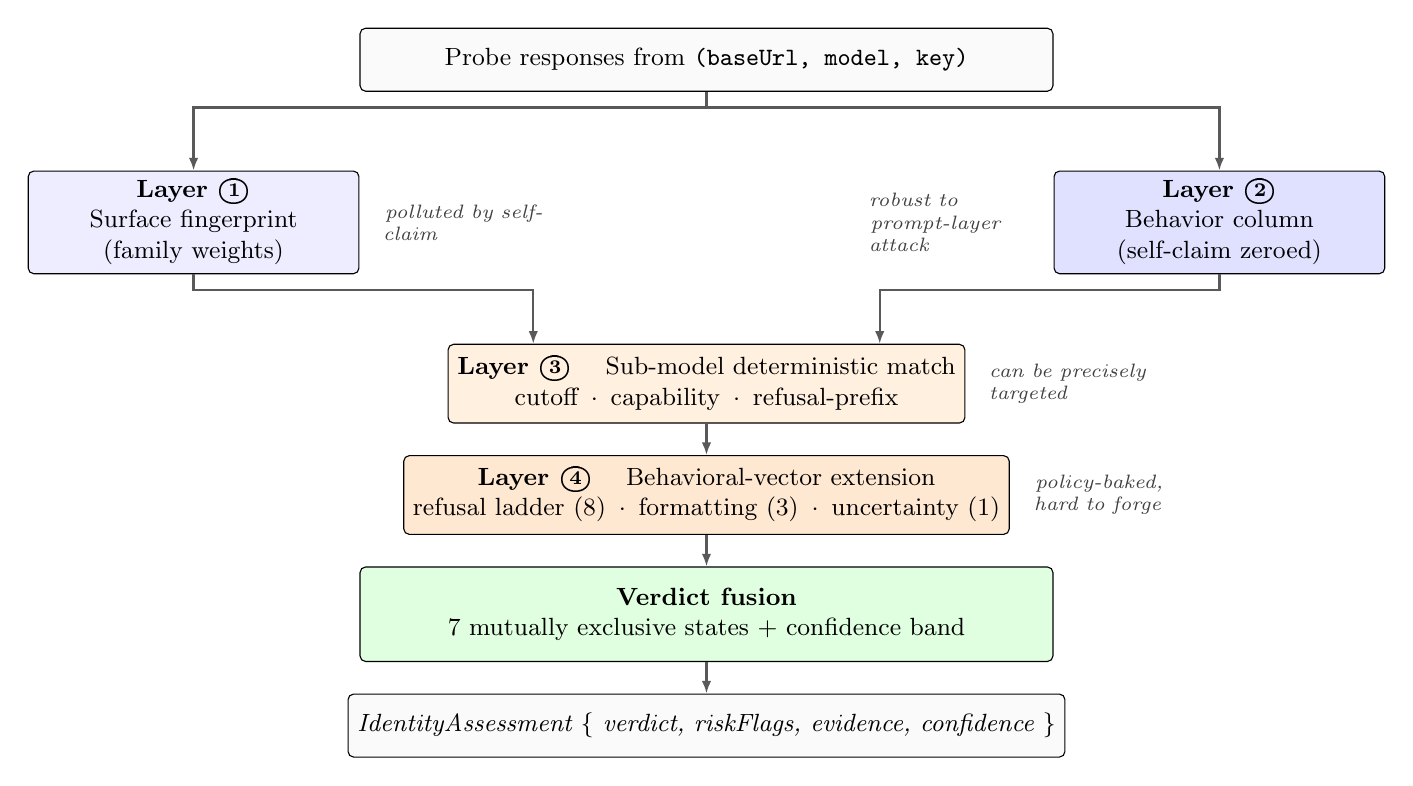
\begin{tikzpicture}[
  node distance=4mm and 6mm,
  every node/.style={font=\small},
  layer/.style={
    draw, rounded corners=2pt,
    minimum width=42mm, minimum height=10mm,
    align=center, fill=gray!8,
  },
  surface/.style={layer, fill=blue!7},
  behavior/.style={layer, fill=blue!12},
  v3/.style={layer, fill=orange!12},
  v3e/.style={layer, fill=orange!18},
  fusion/.style={layer, fill=green!12, minimum width=88mm, minimum height=12mm},
  input/.style={
    draw, rounded corners=2pt,
    minimum width=88mm, minimum height=8mm,
    align=center, fill=gray!4,
  },
  output/.style={
    draw, rounded corners=2pt,
    minimum width=88mm, minimum height=8mm,
    align=center, fill=gray!4,
    font=\small\itshape,
  },
  arrow/.style={-{Latex[length=1.6mm]}, thick, gray!70!black},
  label/.style={font=\scriptsize\itshape, gray!50!black},
]

% Top: input
\node[input] (input) {Probe responses from \texttt{(baseUrl, model, key)}};

% Layer 1 + Layer 2 side by side
\node[surface, below left=10mm and 0mm of input] (l1) {%
  \textbf{Layer \textcircled{\scriptsize 1}}\\Surface fingerprint\\(family weights)};
\node[behavior, below right=10mm and 0mm of input] (l2) {%
  \textbf{Layer \textcircled{\scriptsize 2}}\\Behavior column\\(self-claim zeroed)};

% Layer 3 below
\node[v3, below=10mm of input, yshift=-22mm] (l3) {%
  \textbf{Layer \textcircled{\scriptsize 3}} \quad Sub-model deterministic match\\
  cutoff $\,\cdot\,$ capability $\,\cdot\,$ refusal-prefix};
\path (l3.west) -- node[layer, minimum width=88mm, draw=none, fill=none] {} (l3.east);

% Layer 4 below
\node[v3e, below=4mm of l3] (l4) {%
  \textbf{Layer \textcircled{\scriptsize 4}} \quad Behavioral-vector extension\\
  refusal ladder (8) $\,\cdot\,$ formatting (3) $\,\cdot\,$ uncertainty (1)};

% Verdict fusion
\node[fusion, below=4mm of l4] (fuse) {%
  \textbf{Verdict fusion}\\
  7 mutually exclusive states + confidence band};

% Output
\node[output, below=4mm of fuse] (out) {%
  IdentityAssessment \{ verdict, riskFlags, evidence, confidence \}};

% Arrows
\draw[arrow] (input.south) -- ++(0,-2mm) -| (l1.north);
\draw[arrow] (input.south) -- ++(0,-2mm) -| (l2.north);
\draw[arrow] (l1.south) -- ++(0,-2mm) -| ([xshift=-22mm]l3.north);
\draw[arrow] (l2.south) -- ++(0,-2mm) -| ([xshift=22mm]l3.north);
\draw[arrow] (l3.south) -- (l4.north);
\draw[arrow] (l4.south) -- (fuse.north);
\draw[arrow] (fuse.south) -- (out.north);

% Side annotations
\node[label, right=2mm of l1, anchor=west, text width=20mm] {polluted by self-claim};
\node[label, left=2mm of l2, anchor=east, text width=20mm] {robust to prompt-layer attack};
\node[label, right=2mm of l3, anchor=west, text width=20mm] {can be precisely targeted};
\node[label, right=2mm of l4, anchor=west, text width=20mm] {policy-baked, hard to forge};

\end{tikzpicture}
\caption{The four-layer independent-fingerprint detection architecture (\S\ref{sec:method}).
Each layer uses an independent signal channel; an adversary must simultaneously forge
consistent behavior across multiple channels to escape detection. The verdict fusion
emits one of seven mutually exclusive states with a confidence band.}
\label{fig:architecture}
\end{figure}


\subsection{Layer~\textcircled{1}: Surface fingerprint}\label{sec:layer1}
\textbf{Principle.} The overall textual response (including any
self-identifying language it contains) carries family-discriminative
information at low cost.

\textbf{Implementation.} A linear classifier maps response features to family
weights (Anthropic / OpenAI / Google / xAI / other) with weights pretrained on
known-model traffic.

\textbf{Strength.} Computationally cheap; correct in the vast majority of
unattacked cases.
\textbf{Weakness.} Trivially polluted by self-claim. An adversary need only
inject ``you are Claude Opus 4.7'' into the upstream system prompt to drive
surface output to Anthropic = 100\%. \textbf{Layer~\textcircled{1} must not be
used in isolation.}

\subsection{Layer~\textcircled{2}: Behavior column (self-claim zeroed)}\label{sec:layer2}
\textbf{Principle.} Stripping self-identifying short phrases from the response
and re-classifying yields a column that is largely robust against prompt-layer
self-claim forgery. Adversaries rewrite self-identification far more often
than they rewrite style features.

\textbf{Implementation.} Two parallel classifiers: one over the raw response,
one after regex-deletion of a curated self-identification phrase set.

\textbf{Strength.} Robust against prompt-layer attacks within its band of
confidence.
\textbf{Weakness.} Powerless against pure routing-layer attacks: when the back
end \emph{is} a different family, both columns will agree and indicate the
wrong family relative to the user's claim. Such cases are caught at the
verdict layer by comparing claim against behavior-column truth.

\subsection{Layer~\textcircled{3}: Sub-model deterministic match}\label{sec:layer3}
\textbf{Principle.} Within a family, sibling sub-models (e.g., Claude Opus 4.5
/ 4.6 / 4.7) differ measurably along three observable dimensions: training-data
cutoff, capability boundary, and refusal-prefix style.

\textbf{Implementation.} A baseline database stores, per target model, its
measurements along: \emph{cutoff} (response to ``what is your training-data
cutoff date?''), \emph{capability boundary} (a fixed set of factual questions
including at least one whose answer changes across plausible cutoff dates), and
\emph{refusal prefix} (observed leading text and length when the model refuses
a standardized sensitive request). A heuristic match score selects the
best-matching sub-model when score $\geq 0.60$ and gap to runner-up
$\geq 0.05$; otherwise abstain.

\textbf{Strength.} Strong against pure routing-layer attacks: a different
family scores zero across the board; a different sub-model differs on at
least one dimension.
\textbf{Weakness.} Each dimension can be precisely targeted by a prompt-layer
attack (``your cutoff is 2025-04''); the layer must be paired with
layer~\textcircled{4} for robustness.

\subsection{Layer~\textcircled{4}: Behavioral-vector extension}\label{sec:layer4}
\textbf{Principle.} Layer~\textcircled{3} is augmented with channels that are
harder to forge by system-prompt manipulation. Three vectors:

\begin{itemize}
\item \textbf{Refusal ladder} (8 prompts of monotonically increasing
  sensitivity, from compliant to high-sensitivity, with CBRN material replaced
  by cybercrime equivalents). Each rung is classified
  $\{\text{comply}, \text{partial}, \text{refuse}\}$; the resulting 8-dim
  vector empirically discriminates Claude Opus 4.7 from Anthropic siblings at
  rung L6 (involving methods of self-harm).
\item \textbf{Formatting idiosyncrasy} (3 probes): preferred bullet glyph
  (\texttt{-} / \texttt{*} / \texttt{1.}), markdown header depth, code-block
  language tag.
\item \textbf{Calibrated uncertainty} (1 probe): when asked to express its
  confidence numerically, both the value (e.g., 65\%) and whether the value is
  a round multiple of ten. The latter discriminates same-family siblings such
  as GPT-5.5 (\textsc{isRoundRate}=1.0) from GPT-5.3-codex (\textsc{isRoundRate}=0.33).
\end{itemize}

\textbf{Strength.} Refusal boundaries are determined by the underlying safety
policy and resist system-prompt rewriting; formatting preferences derive from
training distribution rather than runtime instruction; numeric-rounding habits
are highly robust against ``pretend to be confident'' prompt attacks.
\textbf{Weakness.} Twelve additional probes are required.

\subsection{Verdict fusion and seven-state output}\label{sec:verdict}

\begin{table}[h]
\centering
\small
\begin{tabularx}{\linewidth}{@{}lX@{}}
\toprule
Verdict & Trigger (simplified) \\
\midrule
\texttt{clean\_match} & Layers 1, 2, 3 (or 4) all consistent with claim, conf.\ $\geq 0.85$ \\
\texttt{match} & Layers 1, 2 consistent; layer 3 (or 4) abstain or unavailable \\
\texttt{clean\_match\_submodel\_mismatch} & Family consistent but sub-model layer disagrees \\
\texttt{plain\_mismatch} & Behavior-column family $\neq$ claimed family \\
\texttt{mismatch} & Layer 3/4 disagrees with claim at high confidence \\
\texttt{spoof\_selfclaim\_forged} & Self-claim present, behavior-column family differs \\
\texttt{spoof\_behavior\_induced} & Style induced toward claim, layers 3/4 still detect back-end \\
\texttt{ambiguous}/\texttt{uncertain}/\texttt{insufficient\_data} & Insufficient or contradictory signal \\
\bottomrule
\end{tabularx}
\end{table}

% =====================================================================
\section{Engineering Implementation}\label{sec:impl}

The methodology is implemented as an open-source TypeScript library,
\texttt{@bazaarlink/probe-engine}, released under AGPL-3.0 (current version
v0.7.1; see \cref{app:opensource}). The library exposes the four classifiers
as pure functions over recorded HTTP responses, plus a default probe suite of
fixed prompts. A reproducer in possession of the open-source package, an
OpenRouter (or equivalent) API key for baseline construction, and the published
baseline snapshot can independently re-run the evaluation reported in
\cref{sec:results}; no centralized infrastructure is required.

For the field-measurement reported in \cref{sec:field}, the authors operate a
thin Web frontend over the library at \url{https://bazaarlink.ai/probe}. The
frontend accepts a \texttt{(baseUrl, modelId, apiKey)} triple from a submitting
user, executes the probe suite against the supplied endpoint, persists results
to a \texttt{probe\_history} table, and returns the verdict to the submitter.
\textbf{This frontend is a measurement instrument used to collect the field
data; it is not part of the methodology and is not required for reproduction.}

% =====================================================================
\section{Quantitative Results}\label{sec:results}

\subsection{Baseline coverage}\label{sec:baseline}
As of 2026-04-26 the sub-model baseline database contains 27 models across 6
families; 22 have full layer~\textcircled{4} extended-behavior baselines:

\begin{table}[h]
\centering
\small
\begin{tabular}{@{}lrrr@{}}
\toprule
Family & Models & Layer 4 ready & Coverage \\
\midrule
Anthropic & 6 & 6 & 100\% \\
OpenAI & 10 & 10 & 100\% \\
Google & 5 & 5 & 100\% \\
DeepSeek & 2 & 1 & 50\% \\
Qwen & 2 & 0 & 0\% \\
Zhipu & 2 & 0 & 0\% \\
\midrule
\textbf{Total} & \textbf{27} & \textbf{22} & \textbf{81\%} \\
\bottomrule
\end{tabular}
\end{table}

The five missing baselines correspond to families with \emph{zero downstream
claims} during the measurement window; baseline construction is deferred to
conserve compute budget.

\subsection{Synthetic stress test (cost-constrained)}\label{sec:synthetic}
Each round of synthetic testing costs $\approx$~USD~\$0.05. Within budget the
study executed 18 intra-family substitution rounds and 6 genuine-model stress
rounds. We honestly disclose: $n{=}18$ yields a 95\% Wilson confidence interval
of $[74.2\%, 99.0\%]$ --- sample size is \textbf{insufficient to claim a tight
point estimate}.

\begin{table}[h]
\centering
\small
\begin{tabular}{@{}lrr@{}}
\toprule
Condition & $n$ & TP / TN rate \\
\midrule
Intra-family --- naive system prompt & 6 & 6/6 = 100\% \\
Intra-family --- forceful system prompt & 6 & 6/6 = 100\% \\
Intra-family --- injection-mode system prompt & 6 & 5/6 = 83\% \\
\textbf{Intra-family aggregate} & \textbf{18} & \textbf{17/18 = 94.4\%} \\
Genuine model under spoof prompt --- flagged as spoof & 6 & \textbf{0/6 = 0\%} \\
\bottomrule
\end{tabular}
\end{table}

The single missed case was Anthropic Claude Opus 4.6 under injection-mode
attack pushing its L6 refusal boundary to Opus 4.7's level. This is the
layer~\textcircled{4} injection ceiling, addressed in \cref{sec:ceiling}.

\subsection{14-day field deployment}\label{sec:field}

\paragraph{Volume.}
Total probe runs: 625. Distinct \texttt{baseUrl} endpoints: 171. Distinct
claimed \texttt{modelId} values: 47. Admin-verified-clean stamps: 6.

\paragraph{Verdict distribution (n=561 with verdict).}
\begin{table}[h]
\centering
\small
\begin{tabular}{@{}lrr@{}}
\toprule
\texttt{verdict.status} & $n$ & share \\
\midrule
\texttt{clean\_match} & 279 & 49.7\% \\
\texttt{match} & 162 & 28.9\% \\
\texttt{clean\_match\_submodel\_mismatch} & 35 & 6.2\% \\
\texttt{plain\_mismatch} & 35 & 6.2\% \\
\texttt{mismatch} & 14 & 2.5\% \\
\texttt{insufficient\_data} & 11 & 2.0\% \\
\texttt{uncertain} & 7 & 1.2\% \\
\texttt{spoof\_selfclaim\_forged} & 6 & 1.1\% \\
\texttt{spoof\_behavior\_induced} & 6 & 1.1\% \\
\texttt{ambiguous} & 6 & 1.1\% \\
\bottomrule
\end{tabular}
\end{table}

Strict reading: \textbf{12 cases (2.1\%) are high-confidence spoof verdicts}
(the two \texttt{spoof\_*} states combined). Broader reading including
\texttt{plain\_mismatch}, \texttt{mismatch}, and
\texttt{clean\_match\_submodel\_mismatch}: \textbf{100 cases (17.8\%) exhibit
some form of model deviation}. The two spoof states split evenly (6+6),
consistent with the dual attack-surface hypothesis.

\paragraph{Endpoint-level violation distribution.}
Treating each \texttt{baseUrl} as a single endpoint and bucketing by 14-day
violation rate:

\begin{table}[h]
\centering
\small
\begin{tabular}{@{}lrr@{}}
\toprule
Bucket & Endpoints & Cumulative probes \\
\midrule
0\% (clean, $n{\geq}1$) & 142 & 306 \\
$<20\%$ ($n{\geq}5$) & 5 & 106 \\
20--50\% ($n{\geq}5$) & 1 & 57 \\
$\geq 50\%$ ($n{\geq}5$) & 1 & 73 \\
$n{<}5$, ${\geq}1$ violation (low evidence) & 9 & 19 \\
Other & 13 & 64 \\
\bottomrule
\end{tabular}
\end{table}

\textbf{Principal finding (RQ1).} Among the 149 higher-evidence endpoints
($n{\geq}5$), \textbf{7 ($\approx 4.7\%$)} show ${\geq}1$ violation;
\textbf{2 ($\approx 1.3\%$)} show ${\geq}20\%$ sustained violation rate.
Relaxing to $n{\geq}1$, $17/171 \approx 9.9\%$ show ${\geq}1$ violation, but at
this relaxation the impact of one-off false positives cannot be ruled out.

\paragraph{Cost.}
The auxiliary judge LLM used by verdict fusion incurred USD \$1.85 over the
14-day window across 625 runs ($\approx$ \$0.00296 per run).

% =====================================================================
\section{A Taxonomy of Substitution Behavior}\label{sec:taxonomy}

Five categories suffice to organize observed behavior. Each is illustrated by
an anchor case from the field; \cref{sec:cases} provides deep case studies for
R1, R2, and R6.

\subsection{Cross-family impersonation}
Advertise model in $F_a$; route to $F_b$. \textbf{Anchor (R6).} A probe of
\texttt{claude-opus-4-6} returned a response whose behavior-column family
weights placed \texttt{openai} = 0.96; sub-model deterministic match identified
GPT-5.4. Verdict: \texttt{spoof\_behavior\_induced}, high confidence.

\subsection{Intra-family silent downgrade}
Advertise higher-tier; route to cheaper same-family. \textbf{Anchor (R8).}
Multiple probes of \texttt{claude-opus-4-7} stably identified by
layer~\textcircled{4} as Claude Opus 4.6 at score $\geq 0.84$. L6 refusal
pattern and formatting preferences match 4.6.

\subsection{Intra-family silent upgrade}
Advertise lower-tier same-family; route to higher-tier. \textbf{Research
observation.} Upgrade-direction substitution defies the obvious commercial
incentive. Two non-fraudulent explanations are plausible: (a) the reseller's
upstream API key is provisioned only for the higher-tier model; (b)
operational error. \textbf{Anchor (R2).} Multiple probes of
\texttt{claude-opus-4-6} identified the back end as Claude Opus 4.7 at 0.89.

\subsection{Version-tag forgery}
Advertise dated or preview-tagged version; route to same-family neighboring
version. The harm: enterprises pin model versions through dated tags to lock
down behavior across regression tests; tag forgery causes such enterprises to
believe they are pinned while in fact receiving a different training snapshot.
\textbf{Anchor (R2/R3).}

\subsection{Provider behavior injection}
Inject system prompt at upstream that constrains an otherwise general-purpose
model into a narrow domain. The user does receive M, but its behavioral
freedom is silently restricted. \textbf{Anchor.} A ``KIRO (Amazon Q
Developer) detection'' flag activated 23 times across multiple endpoints
during the 14-day window.

\subsection{Endpoint summary}\label{sec:endpoints}

\begin{table}[h]
\centering
\small
\begin{tabular}{@{}lllrrl@{}}
\toprule
Code & Masked domain & --- & $n$ & Viol. & Pattern \\
\midrule
R1 & \texttt{api.1xx.ai} & & 73 & 45 & mixed \\
R2 & \texttt{hbxxx.ai} & & 57 & 20 & upgrade + version forgery \\
R3 & \texttt{yunxx.ai} & & 27 & 5 & version drift \\
R4 & \texttt{api.linxxxxxai.com} & & 26 & 4 & sporadic \\
R5 & \texttt{api.gexxxxxxx.top} & & 7 & 1 & dual-protocol \\
R6 & \texttt{api.axxx.com} & & 6 & 1 & cross-family \\
R7 & \texttt{api.sanxxxxxai.top} & & 4 & 2 & cross-family \\
R8 & \texttt{api.aixxxxxx.com} & & 4 & 1 & downgrade \\
R9 & \texttt{us.noxxxxxx.com} & & 4 & 1 & label forgery \\
R10--R15 & (low evidence) & & 1--2 & 1--2 & various \\
\bottomrule
\end{tabular}
\caption{Endpoints with detected violations during the 14-day window. Codename
order reflects evidence strength. R10--R15 are placed in a low-evidence
cohort and not counted toward the principal point estimates.}
\label{tab:endpoints}
\end{table}

\subsection{Deep case studies}\label{sec:cases}

\paragraph{R1 (\texttt{api.1xx.ai}) --- dynamic-routing cross-family impersonation.}
R1 leads the measurement window in both volume (73 probes) and violation rate
(61.6\%, 45/73), and is the highest-confidence persistent-substitution case in
our data. Two features distinguish R1's behavior: (a) a single advertised model
maps to multiple distinct back-end models across different probes; (b) both
prompt-layer and routing-layer attack surfaces are simultaneously observed at
this endpoint.

Concretely, of five probes claiming \texttt{claude-opus-4-6}, two were
identified as the genuine Claude Opus 4.6 (\texttt{clean\_match}), one as
GPT-5.4, one as GPT-5.4 Mini, and one as a non-Anthropic model whose specific
identity could not be locked down. This distribution is inconsistent with any
single static routing map; it is consistent with \textbf{dynamic load
distribution}: the endpoint dispatches the same advertised claim to whichever
back end is currently available.

R1 also exhibits the most complete prompt-layer forgery observed in our data.
One probe of \texttt{claude-haiku-4-5-20251001} was classified
\texttt{spoof\_behavior\_induced}: behavior-column identified GPT-5.3 Codex
while the response style was being induced toward Claude. A separate probe of
\texttt{gpt-5.3-codex-high} was classified \texttt{spoof\_selfclaim\_forged}:
the response contained an explicit ``I am GPT'' self-identification that was
contradicted by behavior-column family weights. \textbf{Both attack surfaces
co-occurring at one endpoint suggest the operator possesses the engineering
capacity to bypass deterministic sub-model matching (layer~\textcircled{3}),
yet remains caught by the behavioral-vector extension (layer~\textcircled{4}).}

\paragraph{R2 (\texttt{hbxxx.ai}) --- version-tag generalization routing.}
R2 accumulated 57 probes and 20 violations (35.1\%) in the 14-day window. Its
violation profile differs from R1's: R2's back-end models are mostly genuine
within their advertised families (Anthropic / Google), but the endpoint
exhibits a systematic inconsistency in version-tag handling. We name this
pattern \textbf{version-tag generalization routing}: the endpoint accepts
arbitrary sub-model version tags --- including discontinued versions, preview
tags, and date-pinned versions --- and uniformly routes them to the ``most
recent available version'' within the same family.

Six probes of \texttt{claude-opus-4-5-20251101} were classified
\texttt{clean\_match\_submodel\_mismatch}, with behavior column identifying
Claude Opus 4.5 (no date tag); 3 probes of \texttt{claude-sonnet-4-5-20250929}
were uniformly identified as plain Claude Sonnet 4.5; probes of
\texttt{gemini-3-pro-preview} were identified as Gemini 3.1 Pro. Most
strikingly, 3 probes of \texttt{claude-sonnet-4-20250514} (a tag with no
corresponding entry in Anthropic's actual product line) were all routed to
Claude Haiku 4.5 --- a cross-tier substitution that fits neither downgrade nor
upgrade typology cleanly.

\textbf{R2's pattern particularly harms enterprise users who pin behavior to
dated version tags for regression-test stability.} Should Anthropic ever update
the underlying weights for Opus 4.5, R2's downstream users would silently
receive a new training snapshot, invalidating their evaluation criteria
without warning.

\paragraph{R6 (\texttt{api.axxx.com}) --- single-event capture of cross-family substitution.}
R6 accumulated 6 probes and 1 violation (16.7\%) --- below our $n{\geq}5$
evidence threshold. R6 is nonetheless retained as a body-text case because that
single violation supplies a clean, complete evidence chain for the cross-family
impersonation pattern, ideal for illustrating how the methodology captures
such substitutions.

Of 6 probes claiming \texttt{claude-opus-4-6}, 3 returned null verdicts (empty
or parse-failure responses), 2 returned \texttt{clean\_match} against genuine
Claude Opus 4.6, and \textbf{1 returned \texttt{plain\_mismatch} with the
back-end identified as OpenAI GPT-5.4}. The four detection layers reported,
for that single event: (1) surface family weights $\texttt{openai}=0.96$;
(2) behavior column likewise OpenAI-leading; (3) sub-model deterministic match
matched GPT-series cutoff/capability/refusal patterns; and (4) response text
contained marketing tone and disclaimer patterns idiosyncratic to OpenAI GPT
models. \textbf{Four mutually independent evidentiary signals all pointed to
GPT-5.4; the verdict layer accordingly emitted \texttt{plain\_mismatch} at high
confidence.}

R6's pattern represents a third typology distinct from R1's (persistent
dynamic) and R2's (systematic generalization): \textbf{incident-style
substitution}. While the expected harm to any given downstream user is lower
than persistent substitution, its unpredictability defeats any defense based
on long-window averaging --- the user may receive a non-claimed model
precisely on the call that constitutes their commercially critical task.

% =====================================================================
\section{Consumer Harm and Policy Implications}\label{sec:policy}

\subsection{Asymmetric information and quantified harm}
Consumer harm in the resale market does not stem from a single ``quality below
claim'' axis but from compounded asymmetries:

\begin{itemize}
\item \textbf{B1 Quality asymmetry.} Inter-model output-quality differences on
  a fixed prompt are typically imperceptible to ordinary users on
  conversation, copywriting, or translation tasks.
\item \textbf{B2 Version asymmetry.} Enterprises lock prompt engineering and
  evaluation criteria to specific dated model versions; version-tag forgery
  silently invalidates the evaluation criterion.
\item \textbf{B3 Policy asymmetry.} If the reseller strips the upstream model's
  safety system prompt, downstream users may mistake the resulting policy
  relaxation for an inherent feature of the model.
\item \textbf{B4 Litigation asymmetry.} Reseller--buyer relationships rest on
  unilateral terms-of-service; resellers are typically domiciled outside the
  buyer's jurisdiction.
\end{itemize}

By the conservative standard from \cref{sec:field} ($n{\geq}5$, violation rate
${\geq}20\%$), \textbf{at least 1.3\% of currently active reseller endpoints
exhibit persistent substitution}.

\subsection{Why upstream providers cannot solve this alone}
Upstream providers have no effective means to detect substitution at reseller
endpoints. Reasons: (1) upstream sees requests from the reseller's API key with
valid \texttt{model} parameters, cannot distinguish reseller self-use from
sanctioned/impersonated downstream use; (2) the upstream's ledger does not
record what the downstream user was told the model is; (3) banning resellers
contradicts upstream commercial interest; (4) self-claim pollution
\emph{also occurs in upstream providers' own first-party traffic} (a user who
injects ``you are GPT-4'' into Anthropic's official API receives a response
self-identifying as GPT-4). \textbf{Substitution detection in the resale
market cannot rely on upstream providers; it must be supplied by independent
third-party measurement infrastructure}~\cite{akerlof1970lemons}.

\subsection{Three implementable disclosure-duty proposals}
\textbf{D1 --- Routing transparency.} Reseller endpoints should disclose the
actually routed upstream model version in each response's metadata (HTTP
header or non-semantic JSON field). Buyers can then verify alignment between
paid-for model and actual routing. Implementation cost is near zero; D1 must
be mandated by regulation or upstream contract.

\textbf{D2 --- Policy-injection disclosure.} Resellers that inject system
prompts at the upstream layer must disclose this injection's existence and
behavioral impact in their public terms. This is a direct application of
existing consumer-protection law's material-disclosure principles.

\textbf{D3 --- Third-party verification badge.} Reseller endpoints should
permit standardized probing by independent verification organizations and
expose the results as a machine-readable badge.

% =====================================================================
\section{Discussion and Limitations}\label{sec:discussion}

\subsection{Sample composition: voluntary submission as a methodological choice}\label{sec:sample}
The 171 endpoints in this study were not obtained by random sampling from a
reseller directory. They are the set of endpoints submitted by users to a
public verification service over a 14-day window. We treat this not as an
unaddressed bias but as a deliberate methodological choice: the population we
are entitled to draw conclusions about is ``endpoints that some downstream
user had reason to verify,'' not ``all reseller endpoints in
existence''~\cite{paxson2004sound}. The validity claim attached to such data
is correspondingly narrower: our prevalence figures (1.3\% strict, 9.9\%
relaxed) describe \emph{the rate at which user-suspected endpoints turn out
to actually exhibit substitution} --- itself a directly meaningful policy
quantity.

\subsection{Detection ceiling}\label{sec:ceiling}
Layer~\textcircled{4} exhibits a 17\% false-negative rate (1/6) under
injection-mode prompt attacks. The mechanism: when the system prompt explicitly
instructs the model to refuse on category $X$, the model's refusal boundary is
pushed up to approximate that of a higher-tier sibling. Closing this ceiling
requires either (a) channels resistant to system-prompt rewriting (multi-turn
consistency, long-context recall accuracy) or (b) adversarial training across
the system-prompt perturbation space.

\subsection{Synthetic-test sample size}
The 95\% Wilson CI of $[74.2\%, 99.0\%]$ on $n{=}18+6$ is statistically
insufficient to anchor the 94.4\% point estimate. Each additional round costs
$\approx$~\$0.05; reaching $n{=}60$ would cost $\approx$~\$3 --- affordable but
in tension with field-deployment investment. Future work should validate the
synthetic point estimate at higher $n$.

\subsection{Endpoint naming and ethical responsibility}
Codenames R1--R15 with partially masked domains balance: (a) avoiding
asymmetric competitive information injected by this paper into the market; (b)
preserving endpoints' rebuttal and re-test space; (c) protecting the research
team. We further attest: a fraction of probe responses flagged as substitution
may have arisen from the endpoint's defensive response to our adversarial
testing rather than its routine production traffic, especially in the
low-evidence cohort (R10--R15). The current research design cannot fully
discriminate between active reseller substitution and endpoint defensive
routing under detected adversarial testing.

\subsection{Ethical public-interest trade-offs}
The LLM API resale market sits at the intersection of upstream service policy,
restricted-region access policy, and consumer-protection law. The findings
here may be invoked by any party to support its position. The authors
acknowledge this risk and disclaim any precommitment to specific disputes in
any jurisdiction.

\subsection{IRB and ethical self-assessment}\label{sec:irb}
This study does not involve human subjects, human-derived biological material,
or personally identifying data. The objects of measurement are publicly
marketed Internet-accessible HTTP API services. Consequently, no Institutional
Review Board (IRB) approval was sought or required under the human-subjects
research definitions of 45 CFR 46 (Common Rule, U.S.) or comparable
jurisdictional analogues.

In lieu of formal IRB review, the authors performed a self-assessment against
the ACM Code of Ethics: (1.2 \emph{avoid harm}) no DoS, no resource exhaustion,
no billing-bypass, no unauthorized access; (2.3 \emph{respect for rules}) all
measurements via legitimately purchased keys under endpoints' published terms;
(2.6 \emph{competence}) methodology peer-reviewed across the multi-iteration
evolution log, with open-source release enabling external community
verification; (3.1 \emph{public good}) the disclosure-duty proposals are
framed for retail-consumer benefit, not author commercial interest; methodology
released under copyleft (AGPL-3.0). A residual concern --- that the paper's
attention may itself induce reputational harm to specific named endpoints --- is
mitigated by the codename + masking convention adopted here.

% =====================================================================
\section{Conclusion}\label{sec:conclusion}

By means of a four-layer independent-fingerprint detection system applied to
171 LLM API resale endpoints over 14 days, this paper has quantified for the
first time the prevalence and distribution of model substitution in a market
that exists, by economic necessity, in a regulatory gray zone. Under
conservative criteria, \textbf{at least 1.3\% of active endpoints exhibit
persistent substitution}; substitutions sort into five categories
--- cross-family impersonation, silent downgrade, silent upgrade, version-tag
forgery, and behavior injection --- each with a documented anchor case. The
paper analyzes the multi-axis asymmetric-information harm imposed on
downstream buyers from a consumer-protection vantage and proposes three
immediately implementable disclosure duties.

Future work proceeds along three axes: (1) random-sampling market measurement
to eliminate selection bias; (2) closing the detection ceiling by introducing
channels resistant to injection-mode prompt attacks; (3) policy
operationalization advancing the D1/D2/D3 disclosure duties through industry
self-regulation and regulator dialogue.

The LLM API resale market is a gray economy born of access policy in a
present regulatory vacuum; the risks borne by its consumers have, for the
first time, been systematically and quantitatively exposed. The authors hope
this measurement provides a concrete factual basis for market transparency,
consumer protection, and forthcoming regulatory dialogue.

% =====================================================================
\bibliographystyle{plain}
\bibliography{refs}

% =====================================================================
\appendix
\section{Reproducibility via SQL and Open-Source Package}\label{app:sql}

The measurement database is PostgreSQL. Below are the queries that reproduce
\cref{sec:results}'s tables.

\begin{lstlisting}
-- Verdict distribution (last 14d)
SELECT "identityAssessment"->'verdict'->>'status' AS status, COUNT(*) AS n
  FROM probe_history
 WHERE "createdAt" > NOW() - INTERVAL '14 days'
   AND "identityAssessment" IS NOT NULL
 GROUP BY 1 ORDER BY 2 DESC;
\end{lstlisting}

For a CLI-level reproduction:
\begin{lstlisting}
npm install -g @bazaarlink/probe-engine
bazaarlink-probe run \
  --base-url <reseller endpoint> \
  --api-key  <your purchased key> \
  --model    <advertised model id> \
  --baseline-model <baseline lookup id> \
  --output report.json
\end{lstlisting}
Layers~\textcircled{1}, \textcircled{2}, \textcircled{3} and verdict fusion are
reproducible at v0.6.0; layer~\textcircled{4} requires v0.7.0+.

\section{Endpoint Codename Statistics}

In this arXiv version, the full codename--domain mapping is withheld. The
codename--statistics correspondence required to interpret \cref{sec:taxonomy}
is given in \cref{tab:endpoints}. Bona-fide researchers may request the full
mapping via the open-source repository.

\section{Open-Source Implementation Correspondence}\label{app:opensource}

A core subset of the methodology is released under AGPL-3.0 at
\url{https://github.com/Bazaarlinkorg/LLMprobe-engine} as the package
\texttt{@bazaarlink/probe-engine} (latest release v0.7.1 as of this manuscript).

\begin{table}[h]
\centering
\small
\begin{tabular}{@{}lll@{}}
\toprule
Layer & Paper section & Source file \\
\midrule
Surface fingerprint & \cref{sec:layer1} & \texttt{src/fingerprint-extractor.ts} \\
Behavior column & \cref{sec:layer2} & \texttt{src/fingerprint-features-v2.ts} \\
Sub-model deterministic match & \cref{sec:layer3} & \texttt{src/sub-model-classifier-v3.ts} \\
Behavioral-vector extension & \cref{sec:layer4} & \texttt{src/sub-model-classifier-v3e.ts} + \texttt{-v3f.ts} \\
Verdict fusion & \cref{sec:verdict} & \texttt{src/identity-verdict.ts} \\
\bottomrule
\end{tabular}
\end{table}

The open-source release ships with offline baseline snapshots for the 22
models reported in \cref{sec:baseline}, allowing reproduction without
dependency on the authors' SaaS API.

\end{document}
